




\subsection{Exercises}
\begin{enumerate}
\item An experiment results in one of the following sample points:$A,B,C,D$ or $E$

\begin{enumerate}
\item Find P(A) if P(B)=0.1,P(C)=0.3,P(D)=0.2 and P(E)=0.1
\item Find P(A) if P(B)=P(C)=P(D)=P(E)=0.1
\item Find P(A) if P(A)=P(B)=P(C) and P(D)=P(E)=0.2
\end{enumerate}
\item The sample space for an experiment contains five sample points with probabilities as shown in the table.Find the probability of each of the following events:
\begin{center}
\begin{tabular}{|c|c|c|c|c|c|}\hline
Sample Points&1&2&3&4&5\\ \hline
Probabilities&0.3&0.3&0.2&0.05&0.15
 \\ \hline
\end{tabular}
\end{center}
\begin{enumerate}
\item \{Either 1,2,3 or 4 occur\}
\item \{Either 1 or 5 occur\}
\item \{Either 2 does not occur\}
\end{enumerate}

\item Two fair coins are tossed,and the outcome,head or tail,on each coin is observed.
\begin{enumerate}
\item Find samples points in the sample space.
\item What are the probabilities of the sample points in part a.
\item Find the probabilities of each of the following events:
\begin{enumerate}
\item \{exactly two head showing on the two coins\}
\item \{at least one head showing on the two coins\}
\item \{one head and one tail showing on the two coins\}
\end{enumerate}
\end{enumerate}



\item Two balls are drawn at random and without replacement from a box containing two blue balls and two red balls.
\begin{enumerate}
\item List the sample points for this experiment.
\item Assign probabilities to the sample points.
\item Find the probability of the following events:
\begin{enumerate}
\item \{two red balls are drawn\}
\item \{One red and one blue are drawn\}
\item \{two balls with the same color are drawn\}
\end{enumerate}
\item The diagram below describes the sample space of a particular experiment and events A and B.
\begin{enumerate}
\item What is the name of the diagram?
\item Assume the sample points have the same probability.Find P(A),P(B) and P(C) .

\end{enumerate}
\end{enumerate}
%\item Show that if two $n \times n$ matrices $L$, $M$ are symmetric, then so are $L+M$ and $kL$.

\end{enumerate}
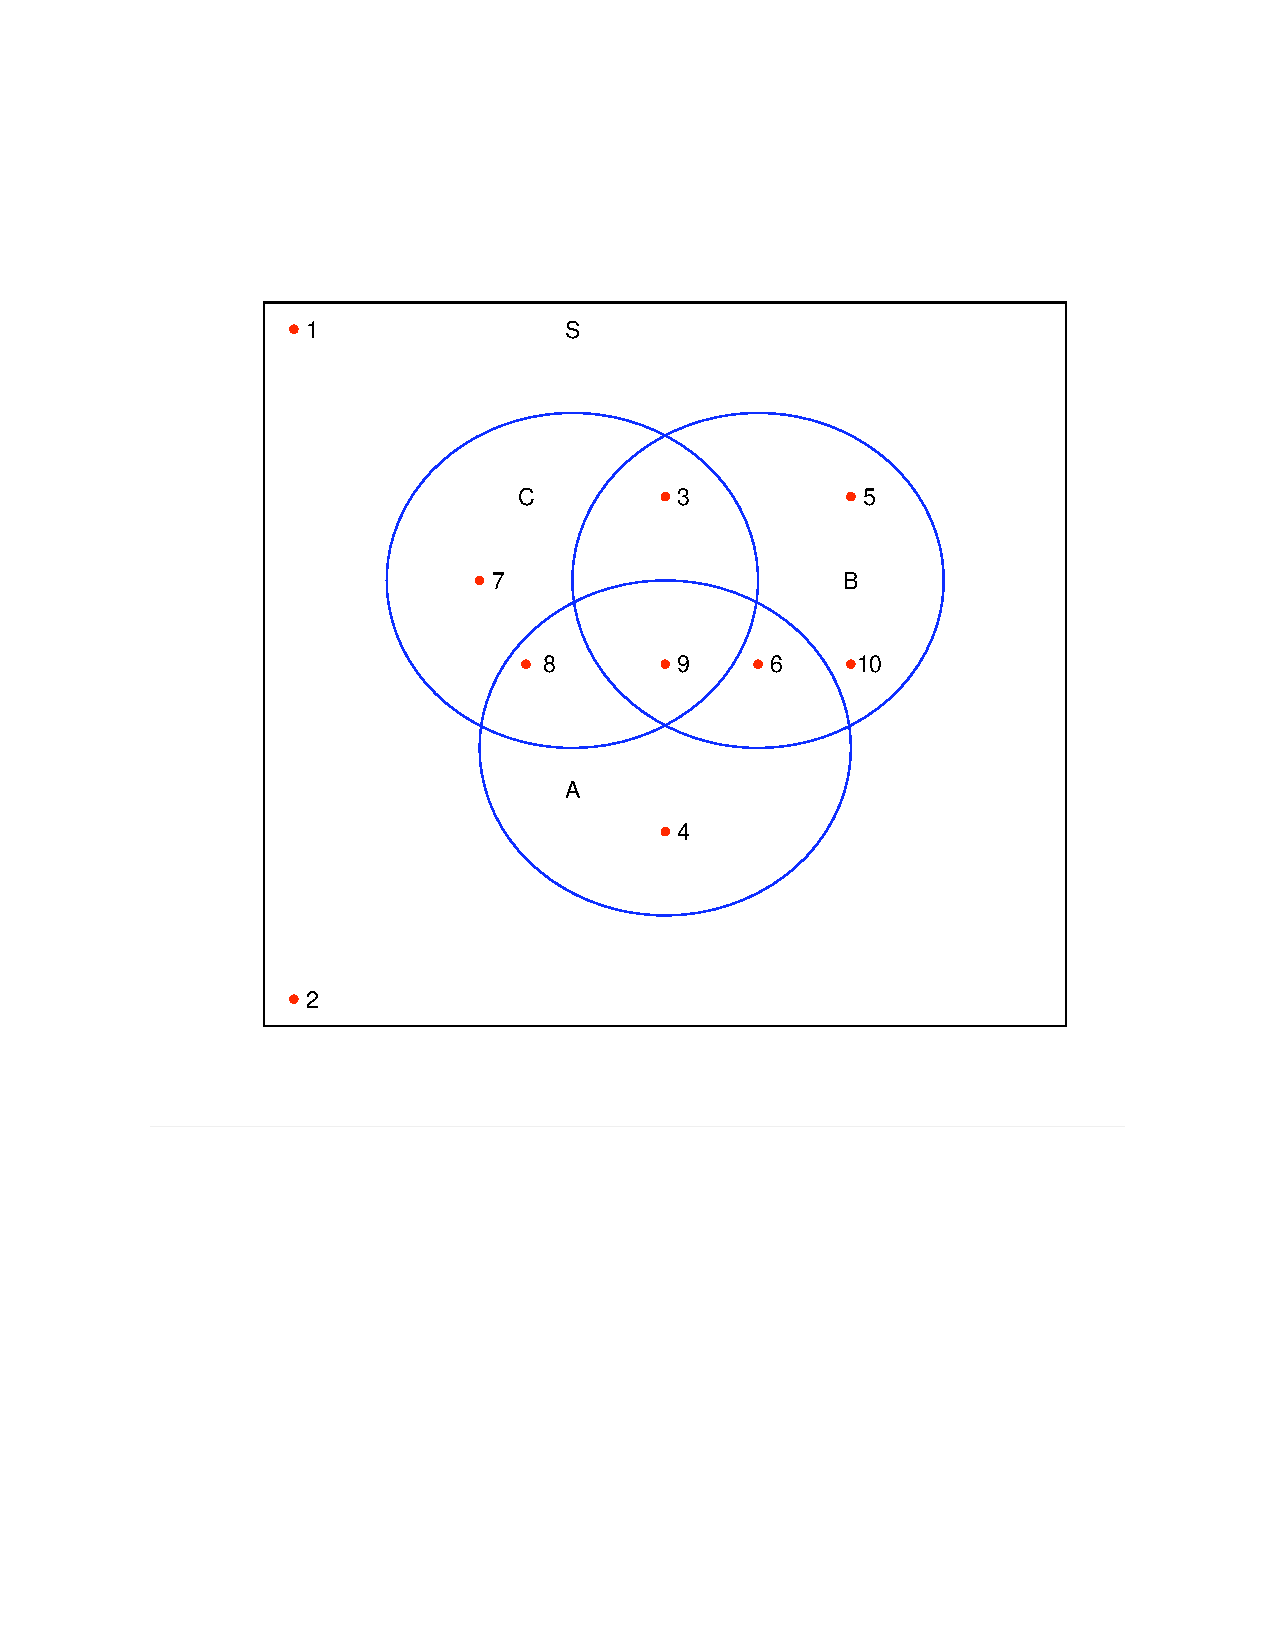
\includegraphics[height=12cm]{Section3/a2-fig-2}
\iffalse
\label{se1} \markright{\ref{se1}
\titleref{se1}}
For the following exercises, let\\ $A=[1\ 2],\ B=\left[
\begin{array}{c}3\\2 \end{array}\right ],\ C=\left [\begin
{array}{rr} 1&-2\\2&-3\end {array} \right ],\ D=\left [\begin
{array}{rr} -2&-5\\1&3\end {array} \right ],\\ E=\left [\begin
{array}{rr} 1&5\\3&8
\\2&1\end {array}\right ],\
F=\left [\begin {array}{rrr} 2&-4&1\\6&-9&1\\4&1&6\\1&7&-5\end {array}\right],\
G=\left [\begin {array}{rrr} 1&2&6\\2&-3&7
\\4&-1&3\end {array}\right ],\\
H=\left [\begin {array}{rrr} 1&0&0\\0&1&0
\\-1&0&0\end {array}\right ],\
I=\left [\begin {array}{rrr} 1&0&0\\0&1&0
\\0&0&1\end {array}\right ],\
K=\left [\begin {array}{rrrr} 1&-2&4&7\\2&3&5&-4
\\1&4&2&1\\-2&1&9&4\end {array}
\right ].$
\bigskip

\begin{enumerate}
\item Which of the following operations are not defined? If they
are defined, what is the size of the resulting matrix
\begin{enumerate}
\item $AC$
\item $CA$
\item $KF^t$
\item $KF$
\item $EB+A^t$
\item $E(H+I)$
\end{enumerate}
\item Find: a) $C+D$\quad b) $D+C$ \quad  c) $G+H$ \quad
d) $D-3C$ \quad e) $2D$
\item Find:
\begin{enumerate} \item $AB$ and $BA$
\item $(C+2D)+BA$ and $C+(2D+BA)$
\item $DC$, $ED$, $(ED)C$ and $E(DC)$
\item $FH+FG$ and $F(G+H)$
\item $G^t$, $H^t$, $(GH)^t$, $G^tH^t$ and $H^tG^t$.
\end{enumerate}
\item Find: $KF$, $FG$ and $FH$.
\item Find tr($K$), tr($I$) and tr($E$).
\item Find $C^3$ and $H^2$.
\item Find $I-H$  and $(I-H)^2$.
\item If $f(x)=x^{2} +2x+2$, $g(x)=x^{2}-x-1$, find
\begin{enumerate} \item $f(C), {\rm (b)}~f(D), {\rm (c)}~g(C), {\rm (d)}~g(D)$.
\end{enumerate}
\item Show that if two $n \times n$ matrices $L$, $M$ are symmetric, then so are $L+M$ and $kL$.

\end{enumerate}



\iffalse
\section{Maple Exercises (optional)}

As in the previous session, first open the linear algebra package.

\begin{maplegroup}
\begin{mapleinput}
\mapleinline{active}{1d}{with(linalg):}{%
}
\end{mapleinput}

\end{maplegroup}
\bigskip

In this chapter, matrix operations and the matrix form of a linear
system ( $A{\bf x}={\bf b}$) were introduced.

We will begin this session by giving a second command to construct
a matrix (the first command was given during the previous Maple
session).

\bigskip

\begin{maplegroup}
\begin{mapleinput}
\mapleinline{active}{1d}{A := matrix(3,3, [1,2,3,2,3,4,3,4,5]);}{%
}
\end{mapleinput}

\mapleresult
\begin{maplelatex}
\[
A :=  \left[ {\begin{array}{rrr} 1 & 2 & 3 \\ 2 & 3 & 4 \\ 3 & 4 &
5
\end{array}}
 \right]
\]
\end{maplelatex}

\end{maplegroup}
\begin{maplegroup}
\begin{mapleinput}
\mapleinline{active}{1d}{B:=matrix(3,3,[2,5,7,13,3,5,6,7,8]);}{%
}
\end{mapleinput}

\mapleresult
\begin{maplelatex}
\[
B :=  \left[ {\begin{array}{rrr} 2 & 5 & 7 \\ 13 & 3 & 5 \\ 6 & 7
& 8
\end{array}}
 \right]
\]
\end{maplelatex}

\end{maplegroup}
\begin{maplegroup}
\begin{mapleinput}
\mapleinline{active}{1d}{C:=matrix(4,3,[1,3,5,7,9,0,8,6,4,2,1,7]);}{%
}
\end{mapleinput}

\mapleresult
\begin{maplelatex}
\[
C :=  \left[ {\begin{array}{rrr} 1 & 3 & 5 \\ 7 & 9 & 0 \\ 8 & 6 &
4 \\ 2 & 1 & 7
\end{array}}
 \right]
\]
\end{maplelatex}

\end{maplegroup}
\begin{maplegroup}
\begin{mapleinput}
\mapleinline{active}{1d}{E:=matrix(3,4,[3,4,7,6,9,2,8,2,6,8,3,12]);}{%
}
\end{mapleinput}

\mapleresult
\begin{maplelatex}
\[
E :=  \left[ {\begin{array}{rrrr} 3 & 4 & 7 & 6 \\ 9 & 2 & 8 & 2
\\ 6 & 8 & 3 & 12
\end{array}}
 \right]
\]
\end{maplelatex}

\end{maplegroup}
\bigskip

{\bf Note:} You can not let a matrix be $D$, a Maple error will
result.

Now that we have a few matrices at hand, we will perform some
matrix operations on them. First, scalar multiplication and matrix
addition. These operations are accomplished using the commands:
scalarmul(\emph{matrix name}, \emph{scalar value}) and
matadd(\emph{matrix name},\emph{matrix name}).

\bigskip

\begin{maplegroup}
\begin{mapleinput}
\mapleinline{active}{1d}{scalarmul(B,2);}{%
}
\end{mapleinput}

\mapleresult
\begin{maplelatex}
\[
 \left[
{\begin{array}{rrr} 4 & 10 & 14 \\ 26 & 6 & 10 \\ 12 & 14 & 16
\end{array}}
 \right]
\]
\end{maplelatex}

\end{maplegroup}
\begin{maplegroup}
\begin{mapleinput}
\mapleinline{active}{1d}{matadd(A , B);}{%
}
\end{mapleinput}

\mapleresult
\begin{maplelatex}
\[
 \left[
{\begin{array}{rrr} 3 & 7 & 10 \\ 15 & 6 & 9 \\ 9 & 11 & 13
\end{array}}
 \right]
\]
\end{maplelatex}

\end{maplegroup}
\bigskip

The `matadd' command can also be used to add scalar multiples of
one matrix to another matrix in the following way.
\bigskip

\begin{maplegroup}
\begin{mapleinput}
\mapleinline{active}{1d}{matadd(3*A,-B);}{%
}
\end{mapleinput}

\mapleresult
\begin{maplelatex}
\[
 \left[
{\begin{array}{rrr} 1 & 1 & 2 \\ -7 & 6 & 7 \\ 3 & 5 & 7
\end{array}}
 \right]
\]
\end{maplelatex}

\end{maplegroup}
\begin{maplegroup}
Matrix multiplication is performed using the `multiply' command.

\end{maplegroup}
\begin{maplegroup}
\begin{mapleinput}
\mapleinline{active}{1d}{multiply(A,B);}{%
}
\end{mapleinput}

\mapleresult
\begin{maplelatex}
\[
 \left[
{\begin{array}{rrr} 46 & 32 & 41 \\ 67 & 47 & 61 \\ 88 & 62 & 81
\end{array}}
 \right]
\]
\end{maplelatex}

\end{maplegroup}
\begin{maplegroup}
\begin{mapleinput}
\mapleinline{active}{1d}{multiply(A,B,E);}{%
}
\end{mapleinput}

\mapleresult
\begin{maplelatex}
\[
 \left[
{\begin{array}{rrrr} 672 & 576 & 701 & 832 \\ 990 & 850 & 1028 &
1228 \\ 1308 & 1124 & 1355 & 1624
\end{array}}
 \right]
\]
\end{maplelatex}

\end{maplegroup}
\bigskip

As shown in the previous section, Maple can be used to solve
systems of equations using the row reduction technique. A second
method uses the `linsolve' command. If we have the system $A{\bf
x}={\bf b}$, this command solves for {\bf x}. This command will be
demonstrated with the matrix $B$ from above, and a row matrix or
vector, $b$.

\bigskip

\begin{maplegroup}
\begin{mapleinput}
\mapleinline{active}{1d}{b:=vector([2,3,6]);}{%
}
\end{mapleinput}

\mapleresult
\begin{maplelatex}
\[
b := [2, \,3, \,6]
\]
\end{maplelatex}

\end{maplegroup}
\begin{maplegroup}
\begin{mapleinput}
\mapleinline{active}{1d}{linsolve(B,b);}{%
}
\end{mapleinput}

\mapleresult
\begin{maplelatex}
\[
 \left[  \! {\displaystyle \frac {29}{119}} , \,{\displaystyle
\frac {260}{119}} , \,{\displaystyle -\frac {160}{119}}  \!
 \right]
\]
\end{maplelatex}

\end{maplegroup}
\bigskip

Try solving the same system using the techniques and commands of
the previous Maple session.

The transpose of a matrix was also defined in this section. On
Maple, the transpose of a matrix is found with the `transpose'
command.
\bigskip

\begin{maplegroup}
\begin{mapleinput}
\mapleinline{active}{1d}{transpose(A);}{%
}
\end{mapleinput}

\mapleresult
\begin{maplelatex}
\[
 \left[
{\begin{array}{rrr} 1 & 2 & 3 \\ 2 & 3 & 4 \\ 3 & 4 & 5
\end{array}}
 \right]
\]
\end{maplelatex}

\end{maplegroup}
\begin{maplegroup}
\mapleresult
\begin{maplettyout}
\end{maplettyout}

\end{maplegroup}
\bigskip

Again you might want to try some other examples for yourself.  You
can also combine the commands to simplify long strings of
calculations. \fi

\section{Answers to activity questions and suggested exercises}
\label{answers2}

{\bf Activity questions}

\bigskip

\noindent {\bf \ref{ssec.arith}:} \quad 1.Yes.

\bigskip

\noindent{\bf \ref{ssec.propma}:} \quad Yes.

\bigskip


\noindent{\bf Suggested exercises}

\begin{enumerate}
\item \begin{enumerate}
\item $1 \times 2$
\item undefined
\item undefined
\item $4 \times 3$
\item undefined
\item undefined \end{enumerate}
\item a) $\left [\begin {array}{rr} -1&-7\\3&0\end {array}
\right ]$
b) $\left [\begin {array}{rr} -1&-7\\3&0\end {array}
\right ]$
c) $\left [\begin {array}{rrr} 2&2&6\\2&-2&7
\\3&-1&3\end {array}\right ]$
\\
d) $\left [\begin {array}{rr} -5&1\\-5&12\end {array} \right ]$ e)
$\left [\begin {array}{rr} -4&-10\\2&6\end {array} \right ]$
\item  \begin{enumerate} \item $7$, $\quad \left [\begin {array}{rr} 3&6\\2&4\end {array} \right ]$
\item $\left [\begin {array}{rr} 0&-6\\6&7\end {array}
\right ]$
\item  $\left [\begin {array}{rrr} -12&19\\7&-11\end {array}
\right ]$,  $\left [\begin {array}{rrr} 3&10\\2&9
\\-3&-7\end {array}\right ]$,  $\left [\begin {array}{rr} 23&-36\\20&-31
\\-17&27\end {array}\right ]$,  $\left [\begin {array}{rr} 23&-36\\20&-31
\\-17&27\end {array}\right ]$
\item $\left [\begin {array}{rrr} -1&11&-13\\-3&29&-24
\\28&0&49\\1&-7&40\end {array}
\right ]$, \quad $\left [\begin {array}{rrr} -1&11&-13\\-3&29&-24
\\28&0&49\\1&-7&40\end {array}
\right ]$
\item $G^t=\left [\begin {array}{rrr} 1&2&4\\2&-3&-1
\\6&7&3\end {array}\right ]$, \quad $H^t=\left [\begin {array}{rrr} 1&0&-1\\0&1&0
\\0&0&0\end {array}\right ]$, \\$(GH)^t=\left [\begin {array}{rrr} -5&-5&1\\2&-3&-1
\\0&0&0\end {array}\right ]$ \\

$G^tH^t=\left [\begin {array}{rrr} 1&2&-1\\2&-3&-2
\\6&7&-6\end {array}\right ]$, \quad $H^tG^t=\left [\begin {array}{rrr} -5&-5&1\\2&-3&-1
\\0&0&0\end {array}\right ]$
\end{enumerate}
\item $KF=\left [\begin {array}{rrr} 13&67&-12\\38&-58&55
\\35&-31&12\\42&36&33\end {array}
\right ]$, \quad  $FG=\left [\begin {array}{rrr}
-2&15&-13\\-8&38&-24
\\30&-1&49\\-5&-14&40\end {array}
\right ]$, \\ $FH=\left [\begin {array}{rrr} 1&-4&0\\5&-9&0
\\-2&1&0\\6&7&0\end {array}\right
]$
\item $10$, $3$, $E$ is not square
\item $C^3=\left [\begin {array}{rr} 5&-6\\6&-7\end {array}
\right ]$,\quad $H^2=\left [\begin {array}{rrr} 1&0&0\\0&1&0
\\-1&0&0\end {array}\right ]$
\item $\left [\begin {array}{rrr} 0&0&0\\0&0&0
\\1&0&1\end {array}\right ]$

\item a) $\left [\begin {array}{rr} 1&0\\0&1\end {array} \right ]$
b) $\left [\begin {array}{rr} -3&-15\\3&12\end {array} \right ]$
c) $\left [\begin {array}{rr} -5&6\\-6&7
\\\end {array}\right ]$
d) $\left [\begin {array}{rr} 0&0\\0&0\end {array} \right ]$

\item $(L+M)^{t}=L^{t}+M^{t}=L+M$, $(kL)^{t}=kL^{t}=kL$.
\end{enumerate}

%\end{document}
\fi 